\documentclass[autodetect-engine, dvi=dvipdfmx, ja=standard, a4paper, 12pt]{bxjsarticle}

\usepackage[dvipdfmx]{graphicx}

\usepackage{amsmath}
\usepackage{amssymb,latexsym,mathtools}
\usepackage{tabularx}
\usepackage{bm}
\usepackage{url}

%サブキャプションを使うとき
\usepackage[hang,small,bf]{caption}
\usepackage[subrefformat=parens]{subcaption}


\usepackage[version=4]{mhchem} %千葉匠追加
\usepackage{multirow}
\usepackage{bm}
\usepackage{physics}
\usepackage{amsmath}
\usepackage{textcomp} % \degree記号のため

% 表の番号のフォーマットを "Table 1" という形式にする
\renewcommand{\tablename}{Table}


% 図の番号のフォーマットを"Fig.1"という形式にする
\renewcommand{\figurename}{Fig.}

% タイトルの読み込み
%
% 卒業論文・発表要旨
% 
%

% 卒業年度(元号で)
\def\年度{令和6年度}

% 論文の種類:本科→卒業論文 専攻科→修了論文
% 以下のどちらかのコメントを外して下さい.
\def\論文種類{機械知能・航空実験II} % 本科の場合
%\def\論文種類{修了論文} % 専攻科

\def\班{A班}

% 発表会日時(要旨用)
%\def\発表会日時{令和5年2月28日}

% 研究題目
\def\研究題目{ファイン3 \\球と平面の接触特性}
\def\研究題目英語{ }

% 副題
%\def\研究題目副{~もげもげに関する考察~}  % 前後に 飾り"~" をつける
\def\研究題目副{ } % 副題がない場合は全角スペース
%\def\研究題目副英語{-- Considering about moge-moge --} % 前後に飾り "--" をつける
\def\研究題目副英語{ }% 副題(英語)がない場合

% 学生氏名,所属等
\def\学籍番号{C2TB1505}
\def\所属{機械知能・航空工学科 \\ファインメカニクスコース 高・松隈研究室} % 機械知能・航空工学科
\def\学生氏名{千葉 匠}
\def\学生氏名英語{TAKUMI CHIBA}  %名字は全て大文字に
\def\共同実験者{シダーサダヌコンダ,川口朋也,蔦森公亨,\\吉村悠太}
%指導教員氏名
%\def\指導教員氏名{ }
%\def\指導教員氏名英語{ }
% タイトル用日付
\def\実験日{2024年11月6日}
\def\レポート提出日付{2024年11月13日} %西暦+月として下さい
\def\連絡先{chiba.takumi.s4@dc.tohoku.ac.jp}




\begin{document}

% タイトル生成
%
% 卒業論文 表紙
%
% 一関高専 機械・知能系 藤原康宣
% 『卒業論文.tex』を処理すると読み込まれて論文の表紙を生成します
% ※このファイルは編集する必要はありません.
%


\begin{titlepage}
    \begin{center}
    \vspace*{20truept}
    {\LARGE \textgt{\年度 \論文種類 \班}}\\
    \vspace*{60truept}
    
    % 題目出力
    {\Huge \textgt{\研究題目}}\\ %研究題目
    \vspace{10truept}
    {\LARGE  \textgt{ \研究題目副} }\\ % 副題
    \vspace{30truept}
    
    %題目(英語)出力
    {\Large \textbf{\研究題目英語}}\\
    {\large \textbf{\研究題目副英語 }}\\
    
    % 学生氏名出力
    \vspace{30truept}
    {\LARGE \textgt{東北大学 \所属}}\\ % 所属
    \vspace{1zw}
    {\Large \textgt{学籍番号 \学籍番号}}\\ % 学籍番号
    \vspace{1zw}
    {\Huge \textgt{\学生氏名}}\\ % 著者
    \vspace{1zw}
    {\Large \textgt{共同実験者 \共同実験者}}\\
    \vspace{3zw}
    
    % 指導教員氏名出力
    %{\LARGE \textgt{指導教員 \指導教員氏名}}\\ % 著者
    %\vspace{3zw}
    
    % 提出日出力
    {\Large \textgt{実験日 \実験日}}\\
    \vspace{1zw}
    % {\Large \textgt{作成日 \作成日}}\\
    % \vspace{1zw}
    {\Large \textgt{提出日 \レポート提出日付}}\\ % 提出日
    \vspace{3zw}
    {\Large \textgt{連絡先 \連絡先}}\\
    \end{center}
    \end{titlepage}


% 目次生成
\tableofcontents 
\clearpage
% 章ごとに別ファイルにして,下さい.
% 各章のファイルは,\input{ファイル名} で読み込んで下さい
%\input{章別サンプル}
\section{目的}

高分子材料は長い分子鎖の集合体から構成される材料であり,材料の巨視的変形挙動は分子鎖の化学構造のみならず,分子鎖の絡合いや配列など,集合体としての高次構造にも強く依存する.そのため,一般的な金属材料とは異なり,応力ひずみ応答における降伏前の非線形粘弾性応答,降伏後のネッキング(局所的なくびれの発生および伝ぱ)を伴うひずみ軟化,ネッキング後の分子鎖配向を原因とするひずみ硬化など,複雑な力学挙動を示す.また,高分子材料は成形時の温度や圧力,流動によって異なる材料微細組織を形成し,力学応答も変化する.本実験では,異なる温度で成形された高分子材料に対して組織観察・引張試験を行い,微視的組織と力学特性の関係について理解を深める.
\section{原理}

\subsection{結晶性熱可塑性高分子材料}
熱すると溶けて冷却すると硬化する高分子材料は熱可塑性高分子材料と呼ばれる.熱可塑性高分子材料でも,硬化する際に分子鎖が秩序をもって配列するものがあり,このような材料は結晶性を有するといわれる.ただし,金属材料のような広範囲の規則正しい配列ではなく,図\ref{fig:crystalline}のような分子鎖が折りたたまった構造となっている.この領域を高分子の結晶相とし,それ以外の不規則に分子鎖が絡まり合った領域は非晶相と呼ばれる.また,一部の結晶性高分子材料は図\ref{fig:階層構造}のような結晶相と非晶相が積み重なり,核から放射状に成長することによって形成される球晶と呼ばれる微細組織を形成する.球晶の大きさはおよそ数十~数百$\mu$m程度であり,偏光顕微鏡観察によって観察することができる(図\ref{fig:球晶構造}).

\begin{figure}[htbp]
    \begin{minipage}[htbp]{0.45\linewidth}
      \centering
      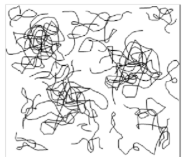
\includegraphics[keepaspectratio, scale=1]{fig/fig_amorphous.png}
      \subcaption{Amorphous polymer}
      \label{fig:amorphous}
    \end{minipage}
    \begin{minipage}[htbp]{0.45\linewidth}
      \centering
      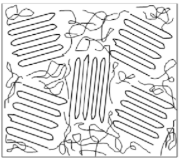
\includegraphics[keepaspectratio, scale=1]{fig/fig_crystalline.png}
      \subcaption{Crystalline polymer}
      \label{fig:crystalline}
    \end{minipage}
    \centering
    \caption{Amorphous and crystalline polymer materialsg.}
    \label{fig:amorphous_crystalline}
\end{figure}

\begin{figure}[htbp]
    \centering %中央揃え
    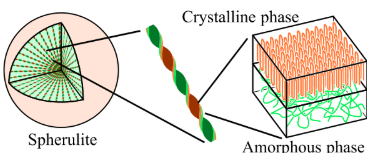
\includegraphics[width=100truemm,clip]{fig/fig_階層構造}
    \caption{Hierarchical structure of spherulite.}
    \label{fig:階層構造}
\end{figure}

\begin{figure}[htbp]
    \centering %中央揃え
    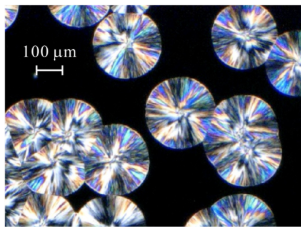
\includegraphics[width=100truemm,clip]{fig/fig_球晶構造}
    \caption{Spherocrystalline structure of polylactic acid.}
    \label{fig:球晶構造}
\end{figure}

\subsection{球晶の形成過程}
球晶が形成される際の核の形成速度$\dot n$と球晶の成長速度$\dot d$は次の式を用いてモデル化されている.ここで$\dot n_0$はエネルギー障壁がないときの核形成速度, $\Delta E_1$は液相中の分子鎖が核になるまでの輸送にかかる運動エネルギー,$R$はBoltzmann定数,$T$は絶対温度,$K_1$は核形成因子パラメータ,$T_m$は完全結晶の融点(平衡融点),はエネルギー障壁がないときの球晶成長速度,$\Delta E_2$は液相中の分子鎖が球晶に組み込まれるまでの輸送にかかる運動エネルギーおよび $K_2$は球晶成長因子パラメータである.式(1),式(2)および実験などから決定される適切なパラメータを用いれば,核形成速度および球晶成長速度が図5のように表される.核形成速度と球晶成長速度が温度によって異なるため,球晶の数や大きさは成形温度に依存する.

\begin{equation}
    \dot n = \dot n_0 \exp \left\{ -\frac{\Delta E_1}{RT} - \frac{K_1 T_m^2}{RT(T_m - T)^2} \right\}
\end{equation}
\begin{equation}
    \dot d = \dot d_0 \exp \left\{ -\frac{\Delta E_2}{RT} - \frac{K_2 T_m^2}{RT(T_m - T)^2} \right\}
\end{equation}

\begin{figure}[htbp]
    \begin{minipage}[htbp]{0.45\linewidth}
      \centering
      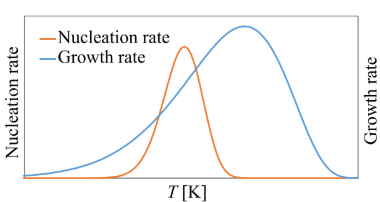
\includegraphics[keepaspectratio, scale=0.7]{fig/fig_模式図.png}
      \subcaption{Schematic diagram}
      \label{fig:模式図}
    \end{minipage}
    \begin{minipage}[htbp]{0.45\linewidth}
      \centering
      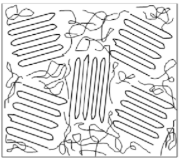
\includegraphics[keepaspectratio, scale=1]{fig/fig_crystalline.png}
      \subcaption{Spherulite growth rate of polypropylene}
      \label{fig:ポリプロピレン成長速度}
    \end{minipage}
    \centering
    \caption{Nucleation rate and spherulite growth rate.}
    \label{fig:核生成速度と成長速度}
\end{figure}
\section{実験装置}
一般的な装置の全体構成の概略を図\ref{fig:装置概略図}に示す.図\ref{fig:装置概略図}に示した装置は,ゴニオメータに X線管ならびに検出器が取り付けられ,試料を固定したままで応力を計測できる.なお,X線管を固定し,検出器や試料をゴニオメータにより走査する形式の装置もある.本実験では,X線管にはCu管を使用し,検出器には2次元位置敏感型検出器を使用して計測した.
\begin{figure}[htbp]
    \centering %中央揃え
    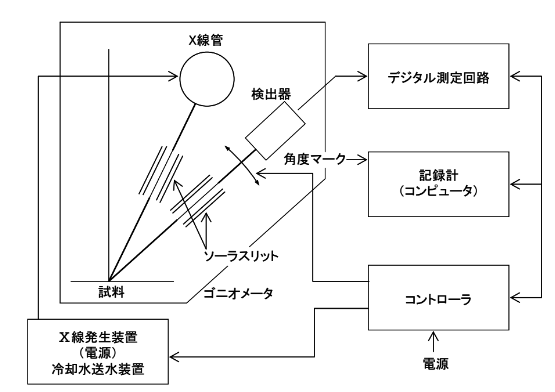
\includegraphics[width=100truemm,clip]{fig/装置概略図.png}
    \caption{Schematic of the overall configuration of a typical device.}
    \label{fig:装置概略図}
\end{figure}
\section{実験方法}
本実験で用いた材料は,(1)高Cr鋼,(2)SUS304ステンレス鋼,(3)銅である.鋼Crフェライト鋼は異なる疲労負荷条件で破断させた試料である.また,オーステナイト系ステンレス鋼は熱処理により,粒界にCr欠乏層が形成された鋭敏化材もの含む.配布された試料に基づき,以下の実験手順で観察を行った.

\subsection{高Cr鋼}
\begin{enumerate}
    \item 機械的研磨\\
          研磨機を用いてバフ研磨を行い試料表面を平坦にした.\\
          荷重:5N\\
          研磨液:ダイアモンド粒径3$\mu$m(1回目)→1$\mu$m(2回目)\\
          研磨時間:300秒\\
          回転数:バフ120rpm\\
                 ヘッド60rpm
    \item 化学的エッチング\\
          ピロ亜硫酸ナトリウム(Na$_2$S$_2$O$_5$)13g,チオ硫酸ナトリウム(Na$_2$S$_2$O$_3$)10g,クエン酸(C$_6$H$_8$O$_7$)1.5g,エタノール5ml,水50mlからなる腐食液を使用した.\\
          エッチング時間:300秒
      \item 光学顕微鏡で表面組織を観察した.
\end{enumerate}

\subsection{SUS304ステンレス鋼}
試験片は(i)MA,(ii)650$^\circ$C2時間,(iii)650$^\circ$C2時間 + 850$^\circ$C2時間の熱処理を施したもので行った.
\begin{enumerate}
      \item 機械的研磨\\
            研磨機を用いてバフ研磨を行い試料表面を平坦にした.\\
            荷重:5N\\
            研磨液:ダイアモンド粒径3$\mu$m(1回目)→1$\mu$m(2回目)\\
            研磨時間:300秒\\
            回転数:バフ120rpm\\
                   ヘッド60rpm
      \item 電気化学エッチング\\
            試験片のエッチング面を陽極として10\%シュウ酸溶液中に入れ,エッチング面積1cm$^2$あたりの電流を1Aに調整して90秒エッチングを行った.1Aにしたときの電圧は5.0Vであった.
      \item 光学顕微鏡で表面組織を観察した.
\end{enumerate}

\subsection{銅}
\begin{enumerate}
    \item ダイアモンドペーストによって機械研磨を行った.
    \item 電解研磨を以下の条件で行った.\\
          電解研磨液:リン酸銅浴(リン酸濃度2/3)\\
          電圧:3.6V\\
          電流:600mA\\
          印加時間:180秒
    \item 光学顕微鏡で表面組織を観察した.
\end{enumerate}
\clearpage
\section{実験結果}

\subsection{ビッカース硬さ試験}
表\ref{tbl:ビッカース硬さ結果}にビッカース硬さの測定結果,表\ref{tbl:ビッカース硬さ平均}にビッカース硬さの平均と標準偏差を示す.

\begin{table}[htbp]
    \centering
    \caption{Vickers hardness test results.}
    \label{tbl:ビッカース硬さ結果}
    \scalebox{0.7}{
    \begin{tabular}{ccccc}
    \hline
    試験回数 & 対角線長さ(横){[}$\mathrm{\mu m}${]} & 対角線長さ(縦){[}$\mathrm{\mu m}${]} & 対角線長さの平均値{[}$\mathrm{\mu m}${]} & ビッカース硬さ$\mathrm{H_v}${[}GPa{]} \\ \hline
    1    & 157.3            & 154.0            & 155.65            & 0.74995            \\ \hline
    2    & 156.0            & 157.8            & 156.90            & 0.73805            \\ \hline
    3    & 157.2            & 154.6            & 155.90            & 0.74755            \\ \hline
    4    & 157.2            & 155.1            & 156.15            & 0.74516            \\ \hline
    5    & 158.4            & 159.2            & 158.80            & 0.72050            \\ \hline
    \end{tabular}
    }
\end{table}

\begin{table}[htbp]
    \centering
    \caption{Mean and standard deviation of Vickers hardness.}
    \label{tbl:ビッカース硬さ平均}
    \scalebox{0.8}{
    \begin{tabular}{ccc}
    \hline
                       & 平均値$\mathrm{H_v}${[}GPa{]} & 標準偏差{[}GPa{]} \\ \hline
    ビッカース硬さ$\mathrm{H_v}${[}GPa{]} & 0.7402         & 0.01190       \\ \hline
    \end{tabular}
    }
\end{table}

\subsection{摩擦試験}

摩擦係数の測定結果をボール試験片の曲率半径$R$ = 1mm,4mm,8mmのそれぞれについて表\ref{tbl:ボール半径1}から表\ref{tbl:ボール半径8}にかけて示す.また,横軸に摩擦係数の平均値$\mu$,縦軸に垂直荷重$W$として測定結果をプロットしたものを図\ref{fig:fig_1mm}から図\ref{fig:fig_8mm}にかけてそれぞれ示す.

どの曲率半径においても,垂直荷重の増加による摩擦係数の変化はほとんど起こっていない.$R$ = 1mmと4mmを比較しても,摩擦係数の変化はほとんど見られない.$R$ = 8mmの場合は,垂直荷重が小さいため,相対的に外乱の影響が大きくなっており,標準偏差が大きくなっている.

\begin{table}[htbp]
    \centering
    \caption{Coefficient of friction measurement results(R=1[mm]).}
    \label{tbl:ボール半径1}
    \scalebox{1.0}{
    \begin{tabular}{cccc}
    \hline
    試験回数 & 0.98{[}N{]} & 4.9{[}N{]} & 9.8{[}N{]} \\ \hline
    1    & 0.676       & 0.673      & 0.656      \\ \hline
    2    & 0.635       & 0.614      & 0.622      \\ \hline
    3    & 0.621       & 0.569      & 0.658      \\ \hline
    4    & 0.564       & 0.56       & 0.71       \\ \hline
    5    & 0.56        & 0.604      & 0.744      \\ \hline
    平均値μ & 0.611       & 0.604      & 0.678      \\ \hline
    標準偏差 & 0.0493      & 0.0448     & 0.0485     \\ \hline
    \end{tabular}
    }
\end{table}
\begin{table}[htbp]
    \centering
    \caption{Coefficient of friction measurement results(R=4[mm]).}
    \label{tbl:ボール半径4}
    \scalebox{1.0}{
    \begin{tabular}{cccc}
    \hline
    試験回数 & 0.98{[}N{]} & 4.9{[}N{]} & 9.8{[}N{]} \\ \hline
    1    & 0.581       & 0.601      & 0.585      \\ \hline
    2    & 0.546       & 0.53       & 0.566      \\ \hline
    3    & 0.557       & 0.495      & 0.625      \\ \hline
    4    & 0.638       & 0.492      & 0.69       \\ \hline
    5    & 0.612       & 0.54       & 0.568      \\ \hline
    平均値μ & 0.587       & 0.532      & 0.607      \\ \hline
    標準偏差 & 0.0382      & 0.0442     & 0.0522     \\ \hline
    \end{tabular}
    }
\end{table}
\begin{table}[htbp]
    \centering
    \caption{Coefficient of friction measurement results(R=8[mm]).}
    \label{tbl:ボール半径8}
    \scalebox{1.0}{
    \begin{tabular}{cccc}
    \hline
    試験回数 & 0.098{[}N{]} & 0.196{[}N{]} & 0.49{[}N{]} \\ \hline
    1    & 0.839        & 0.417        & 0.61        \\ \hline
    2    & 0.454        & 0.418        & 0.61        \\ \hline
    3    & 0.656        & 0.657        & 0.572       \\ \hline
    4    & 0.718        & 0.639        & 0.613       \\ \hline
    5    & 0.558        & 0.693        & 0.542       \\ \hline
    平均値μ & 0.645        & 0.565        & 0.589       \\ \hline
    標準偏差 & 0.148        & 0.136        & 0.0314      \\ \hline
    \end{tabular}
    }
\end{table}

\begin{figure}[htbp]
    \centering %中央揃え
    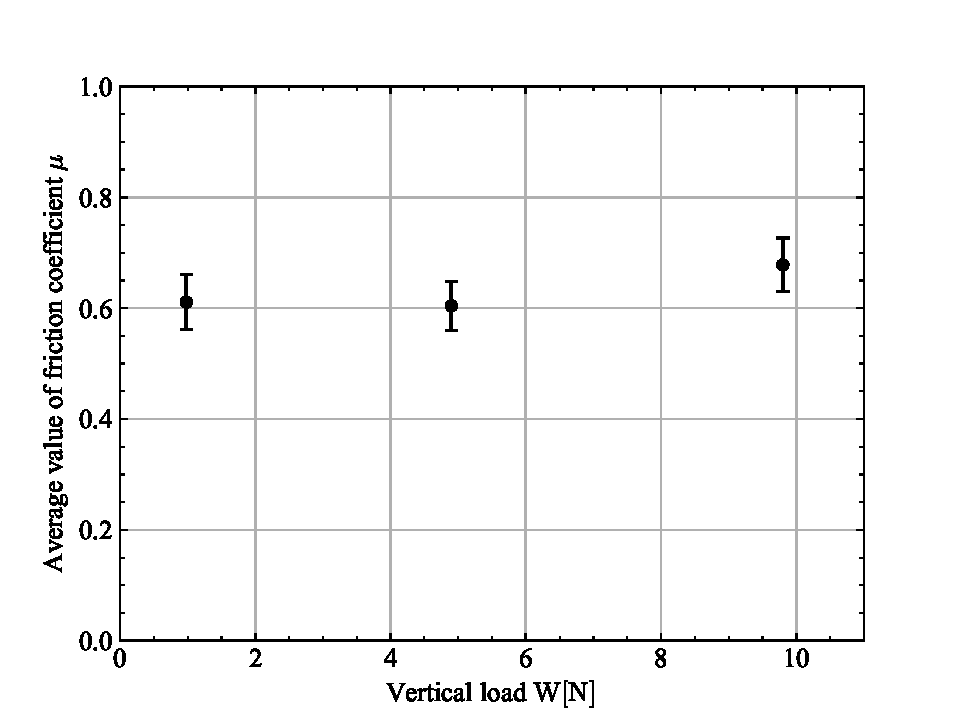
\includegraphics[width=100truemm,clip]{fig/fig_1mm.pdf}
    \caption{Value of coefficient of friction for vertical load(R=1[mm]).}
    \label{fig:fig_1mm}
\end{figure}

\begin{figure}[htbp]
    \centering %中央揃え
    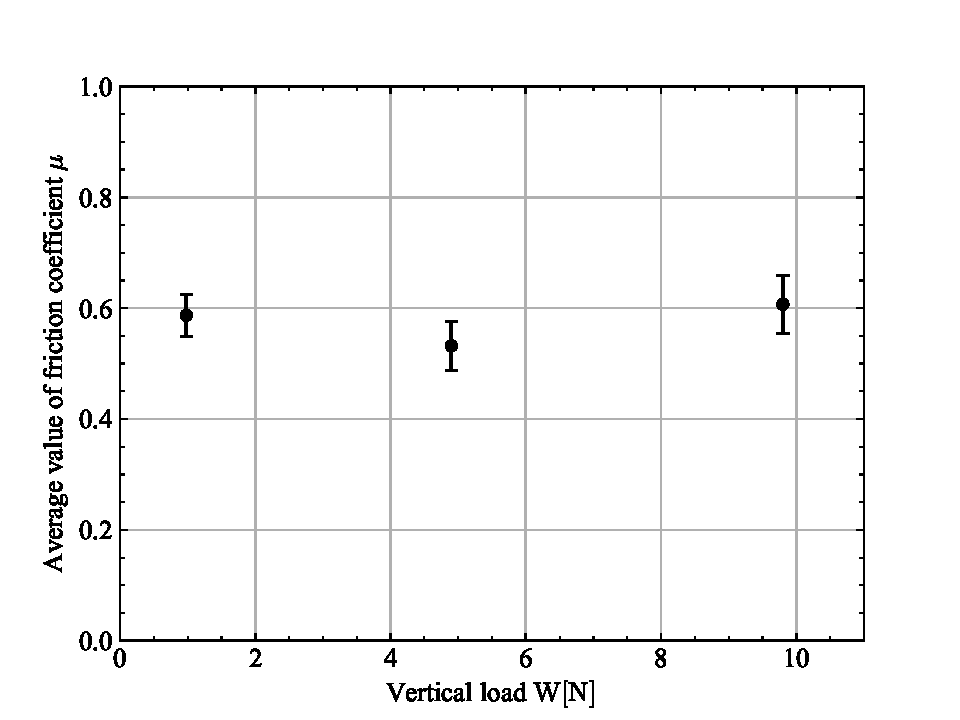
\includegraphics[width=100truemm,clip]{fig/fig_4mm.pdf}
    \caption{Value of coefficient of friction for vertical load(R=4[mm]).}
    \label{fig:fig_4mm}
\end{figure}
\clearpage
\begin{figure}[htbp]
    \centering %中央揃え
    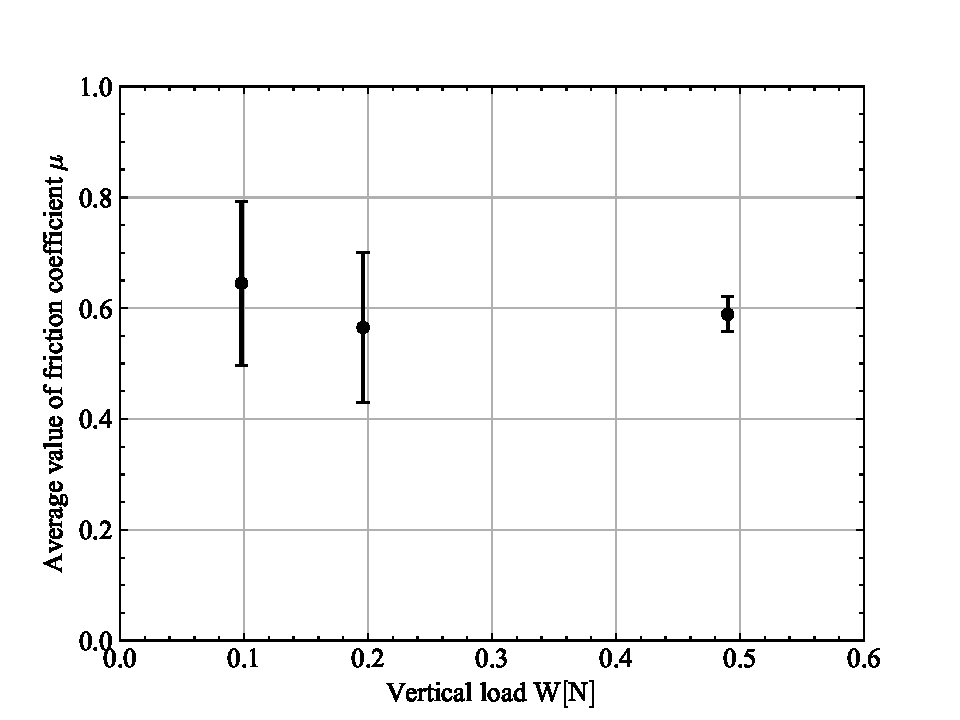
\includegraphics[width=100truemm,clip]{fig/fig_8mm.pdf}
    \caption{Value of coefficient of friction for vertical load(R=8[mm]).}
    \label{fig:fig_8mm}
\end{figure}

\subsection{$\mathrm{P_m/H_v}$値および静的接触形態について}
ヘルツの弾性接触理論を用いて,各摩擦条件における理論上の接触面積$A$,平均接
触圧力$P_m$,$\mathrm{P_m/H_v}$値および静的接触形態を表\ref{tbl:平均圧力1mm}から表\ref{tbl:平均圧力8mm}にかけて示す.

$\mathrm{P_m/H_v}$値を横軸,摩擦係数$\mu$を縦軸としてプロットしたものを図\ref{fig:fig_Pm}に示す.$\mathrm{P_m/H_v}$値の変化による摩擦係数の大きな変化は見られなかった.しかし,おおよその傾向として$\mathrm{P_m/H_v}$ = 0から0.5付近の範囲では値の増加に伴って摩擦係数がやや減少.$\mathrm{P_m/H_v}$ = 0.6から1.3付近の範囲ではは摩擦係数0.6まで増加してほぼ一定の値となり,$\mathrm{P_m/H_v}$ = 1.7で再び増加するグラフとなっている.

\begin{table}[htbp]
    \centering
    \caption{Theoretical contact area, average contact pressure, $\mathrm{P_m/H_v}$ value and static contact morphology(R=1[mm]).}
    \label{tbl:平均圧力1mm}
    \scalebox{1.0}{
    \begin{tabular}{cccc}
    \hline
    垂直荷重 {[}N{]}    & 0.98    & 4.9     & 9.8     \\ \hline
    接触円半径{[}mm{]}   & 0.0234  & 0.0400  & 0.0504  \\ \hline
    接触円面積{[}mm2{]}  & 0.00172 & 0.00503 & 0.00798 \\ \hline
    平均接触圧力{[}GPa{]} & 0.570   & 0.975   & 1.23    \\ \hline
    Pm/Hv           & 0.771   & 1.318   & 1.66    \\ \hline
    静的接触形態          & 弾塑性接触   & 塑性接触    & 塑性接触    \\ \hline
    \end{tabular}
    }
\end{table}

\begin{table}[htbp]
    \centering
    \caption{Theoretical contact area, average contact pressure, $\mathrm{P_m/H_v}$ value and static contact morphology(R=4[mm]).}
    \label{tbl:平均圧力4mm}
    \scalebox{1.0}{
    \begin{tabular}{cccc}
    \hline
    垂直荷重 {[}N{]}    & 0.98    & 4.9    & 9.8    \\ \hline
    接触円半径{[}mm{]}   & 0.0371  & 0.0635 & 0.0800 \\ \hline
    接触円面積{[}mm2{]}  & 0.00433 & 0.0127 & 0.0201 \\ \hline
    平均接触圧力{[}GPa{]} & 0.226   & 0.387  & 0.488  \\ \hline
    Pm/Hv           & 0.306   & 0.523  & 0.659  \\ \hline
    静的接触形態          & 弾性接触    & 弾塑性接触  & 弾塑性接触  \\ \hline
    \end{tabular}
    }
\end{table}

\begin{table}[htbp]
    \centering
    \caption{Theoretical contact area, average contact pressure, $\mathrm{P_m/H_v}$ value and static contact morphology(R=8[mm]).}
    \label{tbl:平均圧力8mm}
    \scalebox{1.0}{
    \begin{tabular}{cccc}
    \hline
    垂直荷重 {[}N{]}    & 0.098   & 0.196   & 0.49    \\ \hline
    接触円半径{[}mm{]}   & 0.0217  & 0.0274  & 0.0371  \\ \hline
    接触円面積{[}mm2{]}  & 0.00148 & 0.00235 & 0.00433 \\ \hline
    平均接触圧力{[}GPa{]} & 0.0662  & 0.0834  & 0.1132  \\ \hline
    Pm/Hv           & 0.0894  & 0.113   & 0.153   \\ \hline
    静的接触形態          & 弾性接触    & 弾性接触    & 弾性接触    \\ \hline
    \end{tabular}
    }
\end{table}

\begin{figure}[htbp]
    \centering %中央揃え
    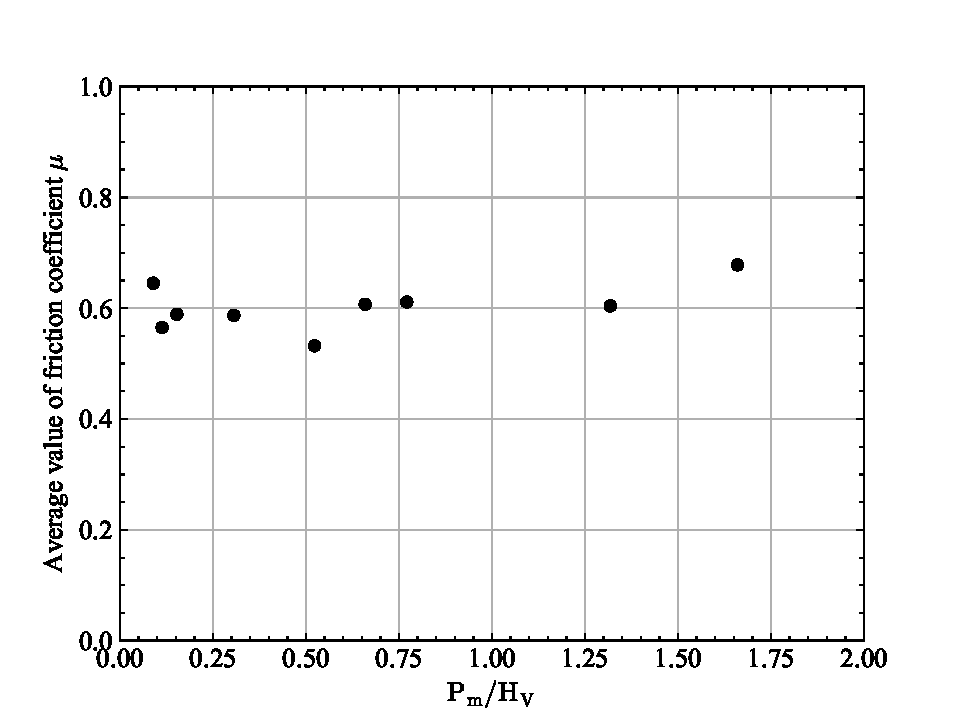
\includegraphics[width=100truemm,clip]{fig/fig_PmHv.pdf}
    \caption{Relationship between coefficient of friction and $\mathrm{P_m/H_v}$ value.}
    \label{fig:fig_Pm}
\end{figure}


\section{課題}

\subsection{(1)異なるセンサによる自律校正}
測定範囲が異なるセンサを用いて今回の自律校正原理を用いる場合を考える.この場合でも,レバーの角度変化を調整することでそれぞれの測定範囲を補うことができ,校正原理を適用することできる.
測定精度が異なるセンサを用いる場合を考えると,式(\ref{eq:誤差Ak-1}),式(\ref{eq:誤差Bk})が同様に成り立つことから,校正原理を適用することができる.

\subsection{(2)レバー倍率の誤差による影響}
レバー系の倍率nに誤差$\Delta$nがあった場合の影響を考察する.式(\ref{eq:誤差Ak-1}),式(\ref{eq:誤差Bk})に$\Delta$n考慮すると,それぞれの誤差は以下のようになる.
式(\ref{eq:倍率誤差Ak-1}),式(\ref{eq:倍率誤差Bk})から,レバー倍率の誤差は,校正曲線の誤差の収束速度に影響を与えることが分かる.レバー倍率の誤差の影響を抑えるためには,nを大きくすることで,$\Delta$nの影響を相対的に小さくすることが有効であると考えられる.

\begin{equation}
    e_{Ak-1} = \frac{e_{A0}}{(n + \Delta n)^{k-1}}
    \label{eq:倍率誤差Ak-1}
\end{equation}
\begin{equation}
    e_{Bk} = \frac{e_{A0}}{(n + \Delta n)^{k}}
    \label{eq:倍率誤差Bk}
\end{equation}

\subsection{(3)センサの平均感度に誤差があった場合の影響}
まずstep1における電圧誤差$E_{A0}$は次式で求められる.
\begin{equation}
    E_{A0} = V_{TrueA} - V_{A0} = V_{TrueA} - S_Ax_{Mea}
    \label{eq:電圧誤差A0}
\end{equation}
次にstep2における電圧誤差$E_{B0}$は次式で求められる.
\begin{equation}
    E_{B0} = T_{TrueB}(\frac{x_{Mea}}{n}) - S_A\frac{x_{Mea}}{n} = E_{A0}
    \label{eq:電圧誤差B0}
\end{equation}
stepkにおける電圧誤差$E_{Bk}$は次式で求められる.
\begin{equation}
    E_{Bk} = T_{TrueB}(\frac{x_{Mea}}{n}) - V_{Bk} = \frac{E_{A0}}{n^k}
    \label{eq:電圧誤差Bk}
\end{equation}

以上から平均感度の誤差は

\begin{thebibliography}{99}
    \bibitem{計測} 高偉,清水裕樹,羽根一博,祖山均,足立幸志. "Bilingual education 計測工学 Measurement and Instrumentation". 朝倉書店 (2020)53-63.
    \bibitem{応力分布} 小山秀夫. "曲げ加工." 軽金属 58.2 (2008): 84-85.
    \bibitem{sokutei} 鈴木金属工業(株) 林博昭."第40回 残留応力測"日本ばね学会 (2024/11/4閲覧)\\
    \url{https://www.jsse-web.jp/kandokoro/kan40.pdf}
    \bibitem{nittetu}日鉄テクノロジー.
    "X線残留応力測定"(2024/11/4閲覧)\\
    \url{https://www.nstec.nipponsteel.com/technology/physical-analysis/structural/structural_02_xrs.html}
    \bibitem{穿孔法} IHI検査計測 三上隆男. "穿孔法による残留応力測定について(その 1)"(2024/11/5閲覧)\\
    \url{https://www.iic-hq.co.jp/library/048/pdf/048_12.pdf}
\end{thebibliography}


\end{document}